% --------------------------------------------------------------
% This is all preamble stuff that you don't have to worry about.
% Head down to where it says "Start here"
% --------------------------------------------------------------
 
\documentclass[11pt]{article}
 
\usepackage[margin=1in]{geometry} 
\usepackage{amsmath,amsthm,amssymb,amsfonts}
\usepackage{tikz}
   \usetikzlibrary{calc,positioning}
   \tikzset{>=latex}
\usepackage{pgfplots}
\usepackage{bm}
\usepackage{xcolor}
\usepackage{units}
\usepackage{floatrow}
\usepackage{times}
\usepackage{epsfig}
\usepackage{graphicx}
\usepackage{subcaption}
% \usepackage[numbered, framed]{mcode}
 
\newcommand{\N}{\mathbb{N}}
\newcommand{\Z}{\mathbb{Z}}
\newcommand{\R}{\mathbb{R}}
 
\newenvironment{theorem}[2][Theorem]{\begin{trivlist}
\item[\hskip \labelsep {\bfseries #1}\hskip \labelsep {\bfseries #2.}]}{\end{trivlist}}
\newenvironment{lemma}[2][Lemma]{\begin{trivlist}
\item[\hskip \labelsep {\bfseries #1}\hskip \labelsep {\bfseries #2.}]}{\end{trivlist}}
\newenvironment{exercise}[2][Exercise]{\begin{trivlist}
\item[\hskip \labelsep {\bfseries #1}\hskip \labelsep {\bfseries #2.}]}{\end{trivlist}}
\newenvironment{reflection}[2][Reflection]{\begin{trivlist}
\item[\hskip \labelsep {\bfseries #1}\hskip \labelsep {\bfseries #2.}]}{\end{trivlist}}
\newenvironment{proposition}[2][Proposition]{\begin{trivlist}
\item[\hskip \labelsep {\bfseries #1}\hskip \labelsep {\bfseries #2.}]}{\end{trivlist}}
\newenvironment{corollary}[2][Corollary]{\begin{trivlist}
\item[\hskip \labelsep {\bfseries #1}\hskip \labelsep {\bfseries #2.}]}{\end{trivlist}}
 
\begin{document}
 
% --------------------------------------------------------------
%                         Start here
% --------------------------------------------------------------
 
%\renewcommand{\qedsymbol}{\filledbox}
 
\title{Model Predictive Control\\
    Programming Exercise - Report} %replace X with the appropriate number
\author{Gian Andrea M{\"u}ller (14-935-035)\\
    Kevin Anschau Schwarzer (12-914-735)\\
    Ueli Eugen Wechsler (11-920-444)} %replace with your name
%if necessary, replace with your course title

\maketitle

\subsection*{Nonlinear model and linearization} % (fold)
\label{sub:nonlinear_model_and_linearization}

\begin{enumerate}
    % 1.
    \item
\end{enumerate}
% subsection nonlinear_model_and_linearization (end)


\subsection*{First MPC controller} % (fold)
\label{sub:first_mpc_controller}

\begin{enumerate}
    \setcounter{enumi}{1}
    % 2.
    \item

    % 3.
    \item The response of the first MPC controller can be seen in
    Figure~\ref{fig:1st_mpc_controller}.
    \begin{figure}[ht]
        \centering
        \begin{subfigure}[c]{0.3\linewidth}
            \centering
            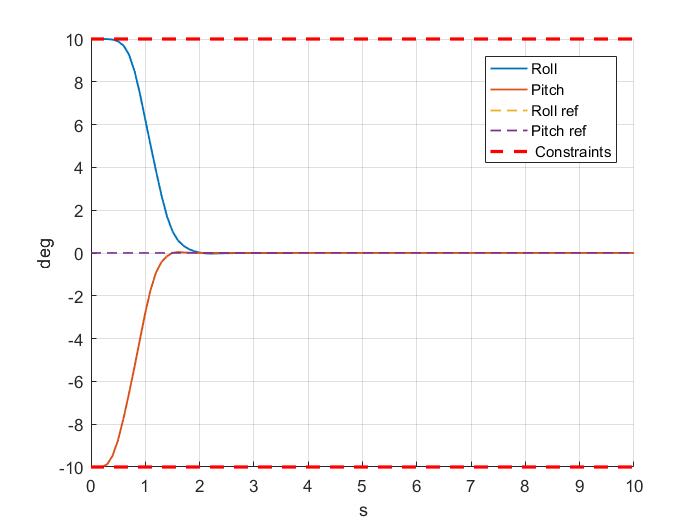
\includegraphics[width=\linewidth]{Plots_03_FirstMPCController/01}
            \caption{Roll- and Pitch}
        \end{subfigure}
        ~
        \begin{subfigure}[c]{0.3\linewidth}
            \centering
            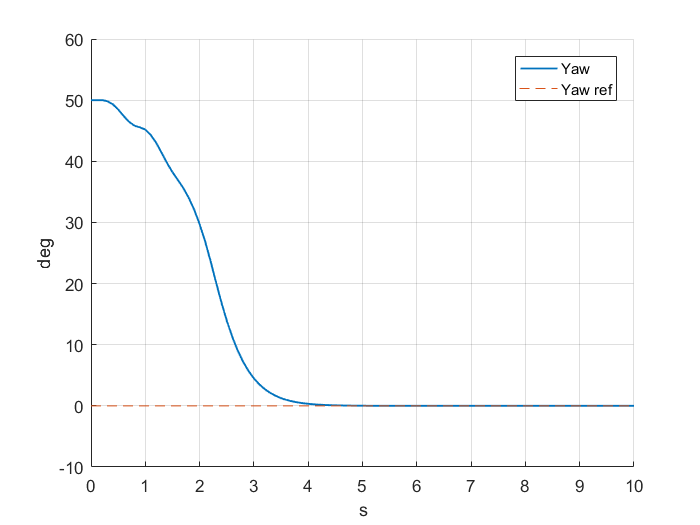
\includegraphics[width=\linewidth]{Plots_03_FirstMPCController/02}
            \caption{Yaw}
        \end{subfigure}
        ~
        \begin{subfigure}[c]{0.3\linewidth}
            \centering
            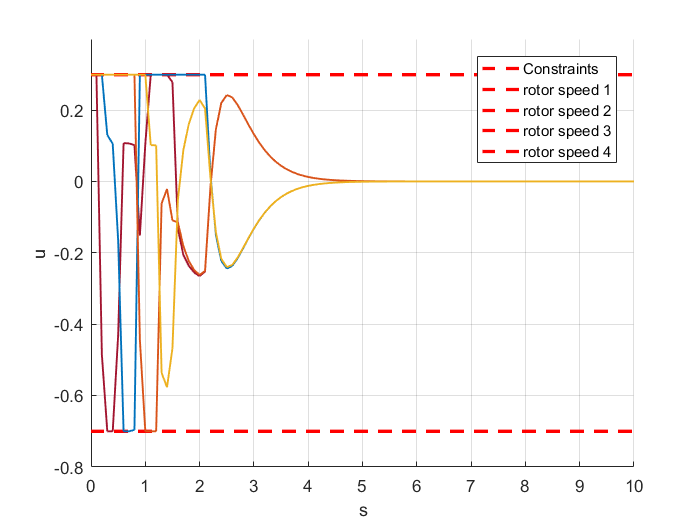
\includegraphics[width=\linewidth]{Plots_03_FirstMPCController/03}
            \caption{Rotor Speeds}
        \end{subfigure}

        \begin{subfigure}[c]{0.3\linewidth}
            \centering
            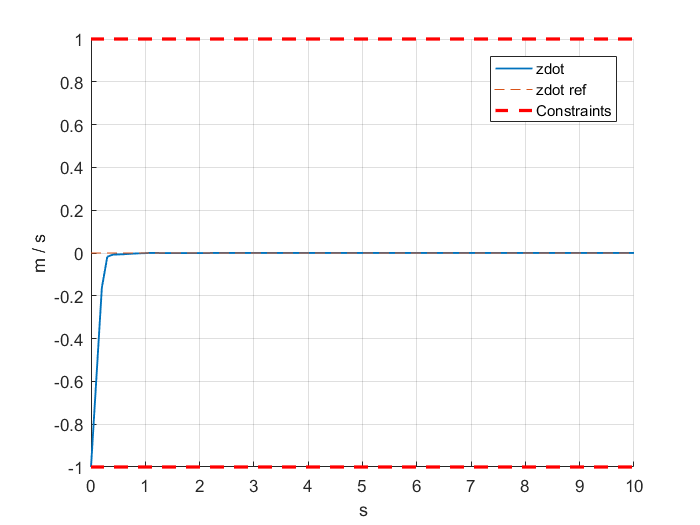
\includegraphics[width=\linewidth]{Plots_03_FirstMPCController/04}
            \caption{zdot}
        \end{subfigure}
        ~
        \begin{subfigure}[c]{0.3\linewidth}
            \centering
            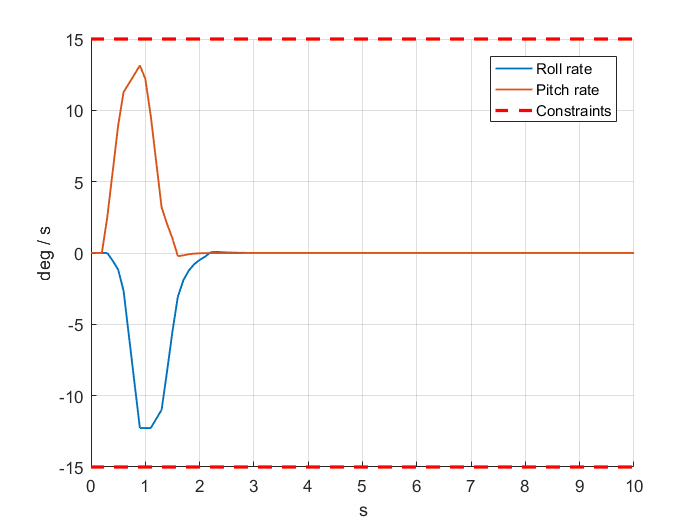
\includegraphics[width=\linewidth]{Plots_03_FirstMPCController/05}
            \caption{Roll and Pitch rates}
        \end{subfigure}
        ~
        \begin{subfigure}[c]{0.3\linewidth}
            \centering
            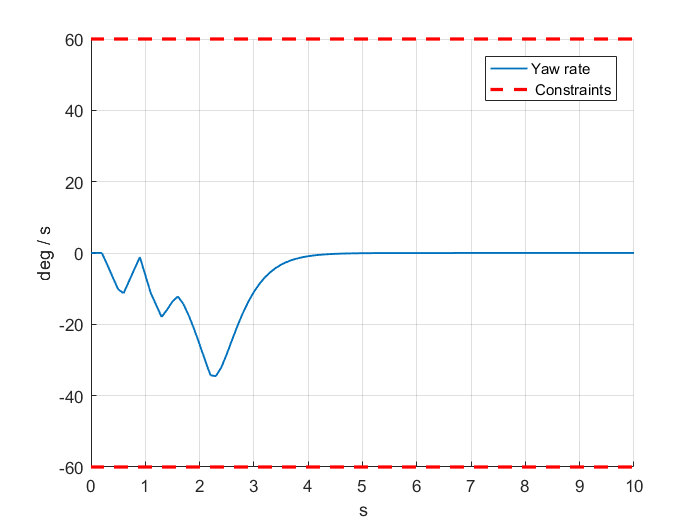
\includegraphics[width=\linewidth]{Plots_03_FirstMPCController/06}
            \caption{Yaw rate}
        \end{subfigure}
        \caption{Response of first MPC controller.}
        \label{fig:1st_mpc_controller}
    \end{figure}
\end{enumerate}

% subsection first_mpc_controller (end)


\subsection*{Reference Tracking} % (fold)
\label{sub:reference_tracking}

\begin{enumerate}
    \setcounter{enumi}{3}
    % 4.
    \item

    % 5.
    \item The response for the constant reference signal can be seen in
    Figure~\ref{fig:constant_reference_with_offset}.
    \begin{figure}[ht]
        \centering
        \begin{subfigure}[c]{0.3\linewidth}
            \centering
            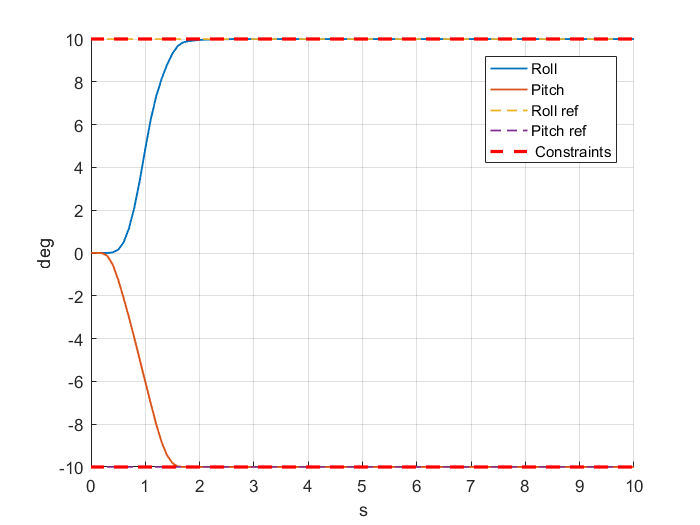
\includegraphics[width=\linewidth]{Plots_05_ReferenceTracking_Constant/01}
            \caption{Roll and Pitch}
        \end{subfigure}
        ~
        \begin{subfigure}[c]{0.3\linewidth}
            \centering
            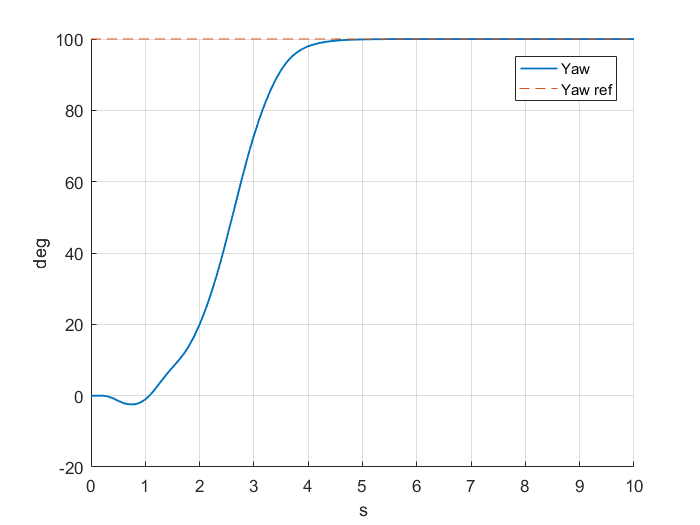
\includegraphics[width=\linewidth]{Plots_05_ReferenceTracking_Constant/02}
            \caption{Yaw}
        \end{subfigure}
        ~
        \begin{subfigure}[c]{0.3\linewidth}
            \centering
            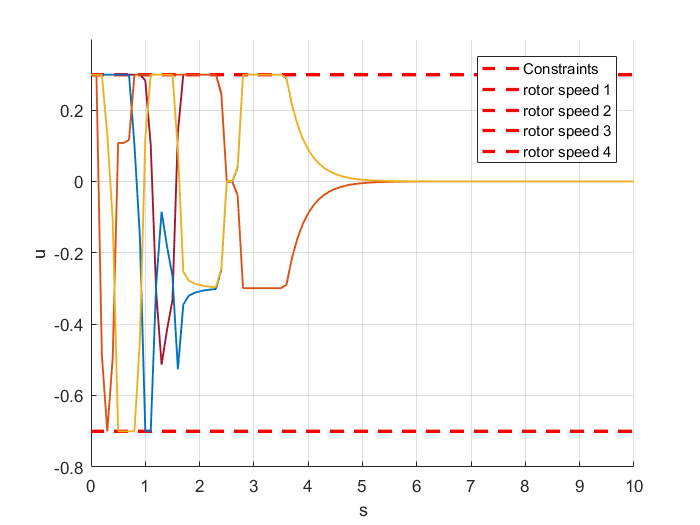
\includegraphics[width=\linewidth]{Plots_05_ReferenceTracking_Constant/03}
            \caption{Rotor Speeds}
        \end{subfigure}

        \begin{subfigure}[c]{0.3\linewidth}
            \centering
            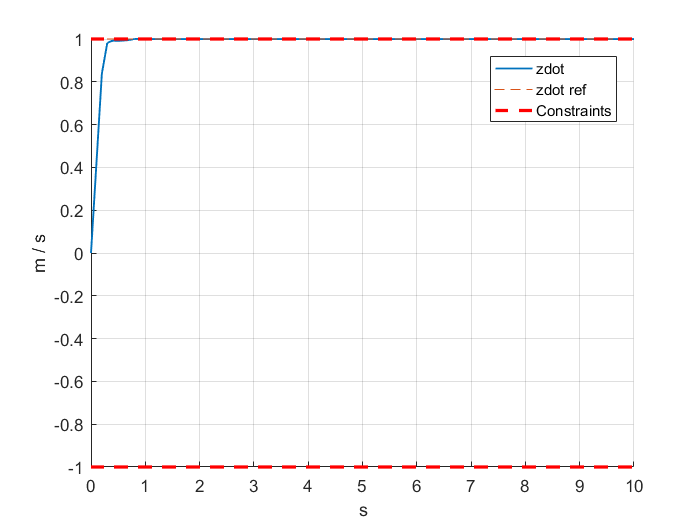
\includegraphics[width=\linewidth]{Plots_05_ReferenceTracking_Constant/04}
            \caption{zdot}
        \end{subfigure}
        ~
        \begin{subfigure}[c]{0.3\linewidth}
            \centering
            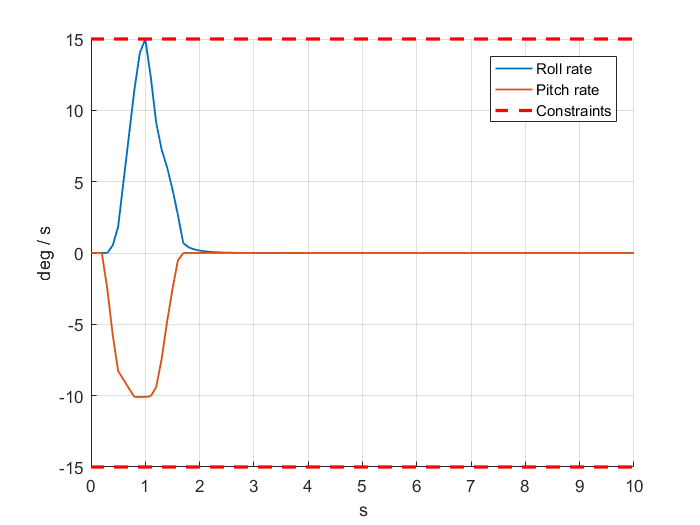
\includegraphics[width=\linewidth]{Plots_05_ReferenceTracking_Constant/05}
            \caption{Roll and Pitch rates}
        \end{subfigure}
        ~
        \begin{subfigure}[c]{0.3\linewidth}
            \centering
            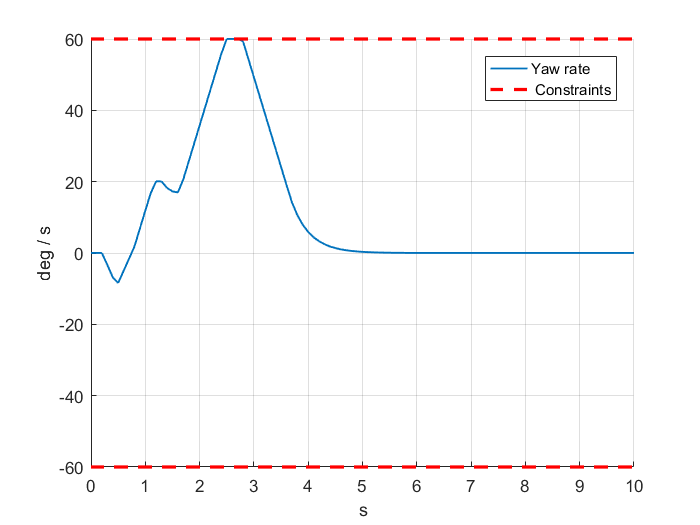
\includegraphics[width=\linewidth]{Plots_05_ReferenceTracking_Constant/06}
            \caption{Yaw rate}
        \end{subfigure}
        \caption{Response for constant reference signal with offset.}
        \label{fig:constant_reference_with_offset}
    \end{figure}

    % 6.
    \item The response for the slowly varying reference signal can be seen in
    Figure~\ref{fig:varying_reference_with_offset}.
    \begin{figure}[ht]
        \centering
        \begin{subfigure}[c]{0.3\linewidth}
            \centering
            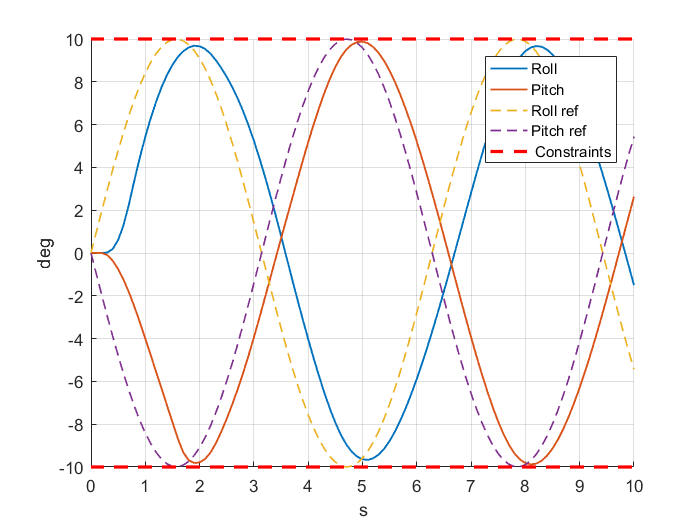
\includegraphics[width=\linewidth]{Plots_06_ReferenceTracking_Varying/01}
            \caption{Roll and Pitch}
        \end{subfigure}
        ~
        \begin{subfigure}[c]{0.3\linewidth}
            \centering
            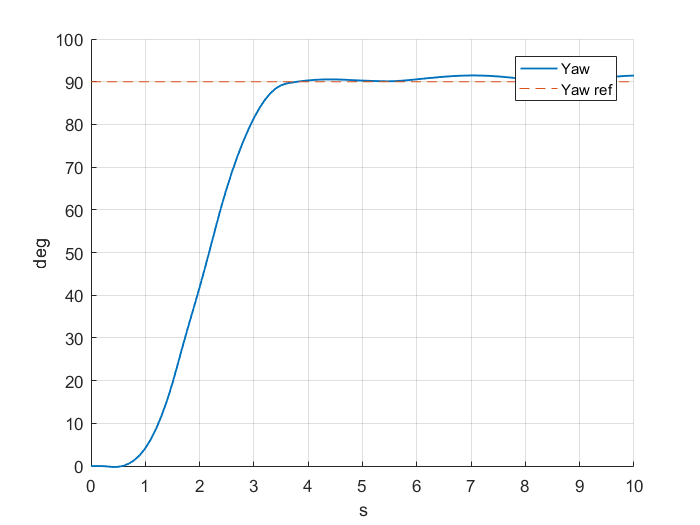
\includegraphics[width=\linewidth]{Plots_06_ReferenceTracking_Varying/02}
            \caption{Yaw}
        \end{subfigure}
        ~
        \begin{subfigure}[c]{0.3\linewidth}
            \centering
            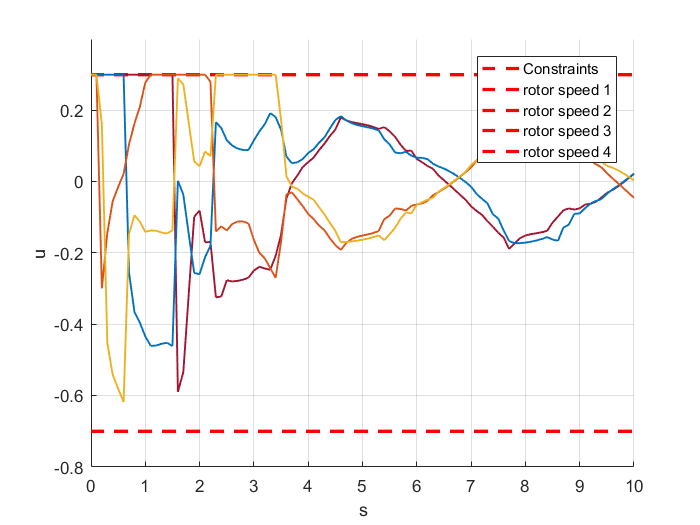
\includegraphics[width=\linewidth]{Plots_06_ReferenceTracking_Varying/03}
            \caption{Rotor Speeds}
        \end{subfigure}

        \begin{subfigure}[c]{0.3\linewidth}
            \centering
            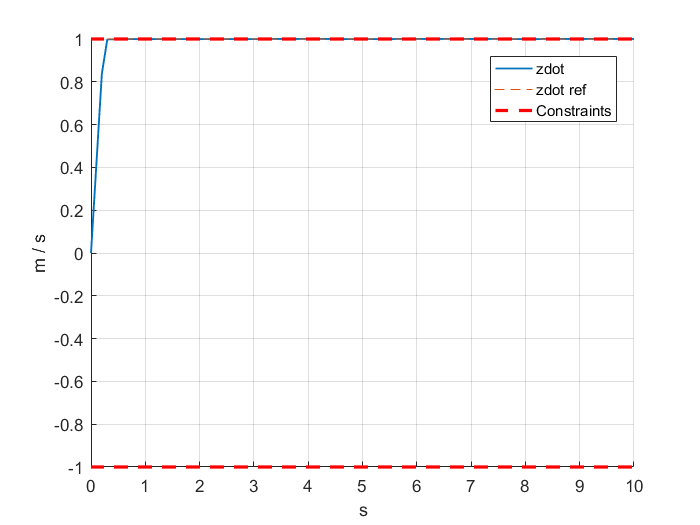
\includegraphics[width=\linewidth]{Plots_06_ReferenceTracking_Varying/04}
            \caption{zdot}
        \end{subfigure}
        ~
        \begin{subfigure}[c]{0.3\linewidth}
            \centering
            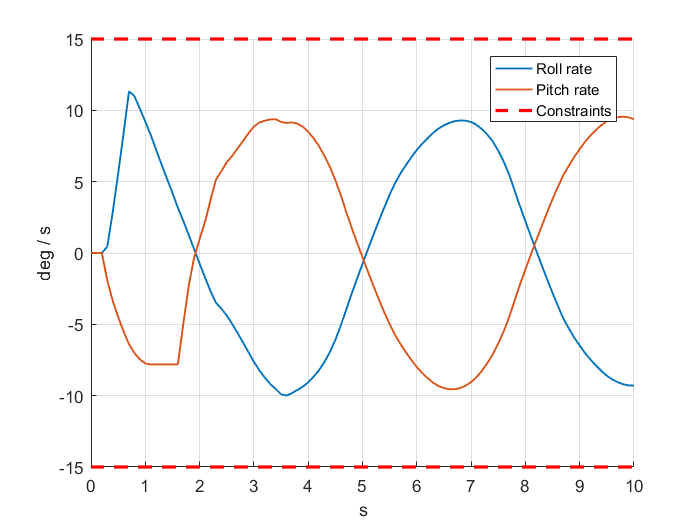
\includegraphics[width=\linewidth]{Plots_06_ReferenceTracking_Varying/05}
            \caption{Roll and Pitch rates}
        \end{subfigure}
        ~
        \begin{subfigure}[c]{0.3\linewidth}
            \centering
            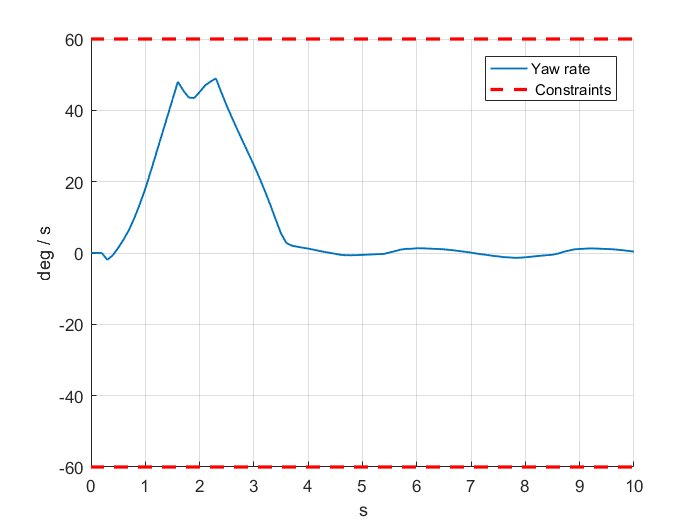
\includegraphics[width=\linewidth]{Plots_06_ReferenceTracking_Varying/06}
            \caption{Yaw rate}
        \end{subfigure}
        \caption{Response for slowly varying reference signal with offset.}
        \label{fig:varying_reference_with_offset}
    \end{figure}
\end{enumerate}

% subsection reference_tracking (end)


\subsection*{First simulation of the nonlinear model} % (fold)
\label{sub:first_simulation_of_the_nonlinear_model}

\begin{enumerate}
    \setcounter{enumi}{6}
    % 7.
    \item The response of the reference tracking of the nonlinear model can be
    seen in Figure~\ref{fig:nonlinear_reference_tracking_with_offset}.
    \begin{figure}[ht]
        \centering
        \begin{subfigure}[c]{0.3\linewidth}
            \centering
            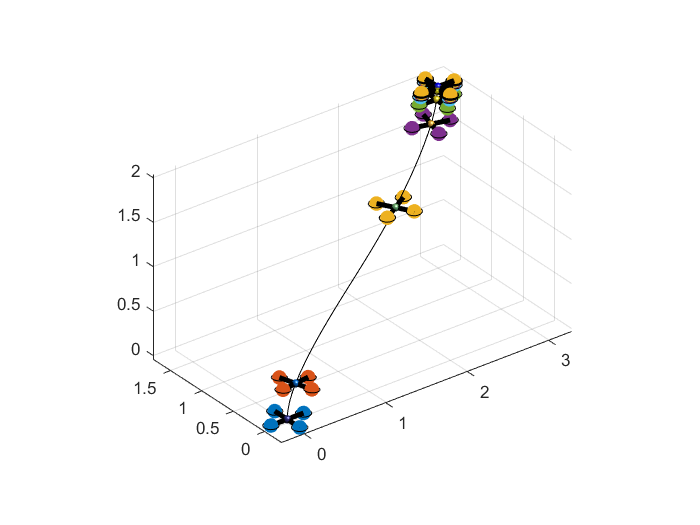
\includegraphics[width=\linewidth]{Plots_07_NonlinearModel_ReferenceTracking/01}
            \caption{Quadrotor}
        \end{subfigure}
        ~
        \begin{subfigure}[c]{0.3\linewidth}
            \centering
            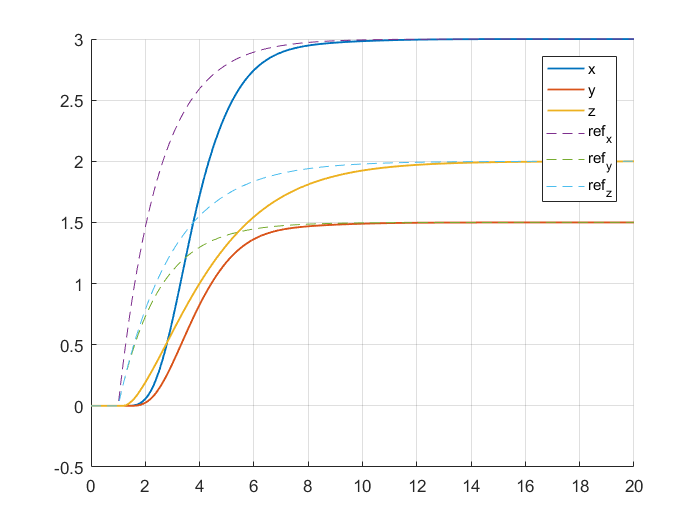
\includegraphics[width=\linewidth]{Plots_07_NonlinearModel_ReferenceTracking/02}
            \caption{x, y and z}
        \end{subfigure}
        ~
        \begin{subfigure}[c]{0.3\linewidth}
            \centering
            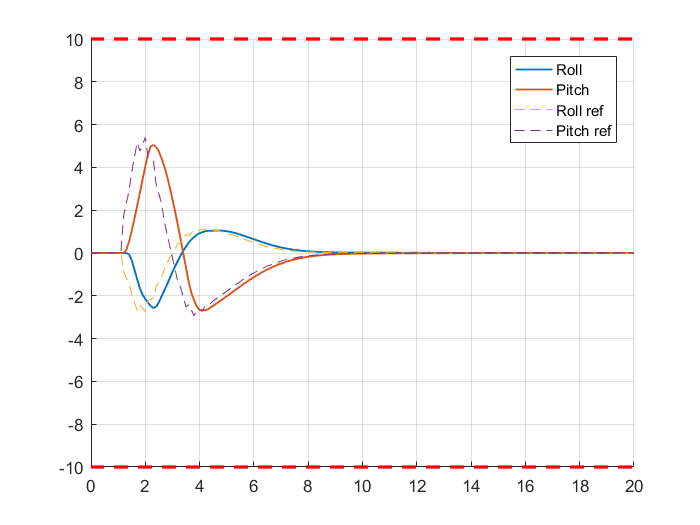
\includegraphics[width=\linewidth]{Plots_07_NonlinearModel_ReferenceTracking/03}
            \caption{Roll and Pitch}
        \end{subfigure}

        \begin{subfigure}[c]{0.3\linewidth}
            \centering
            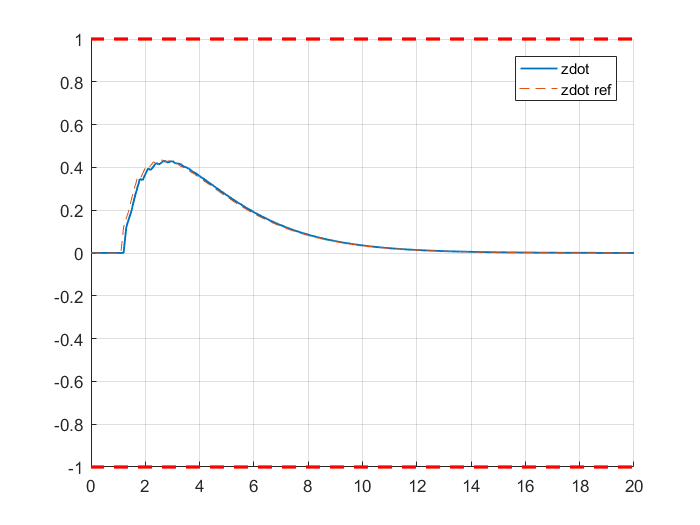
\includegraphics[width=\linewidth]{Plots_07_NonlinearModel_ReferenceTracking/04}
            \caption{zdot}
        \end{subfigure}
        ~
        \begin{subfigure}[c]{0.3\linewidth}
            \centering
            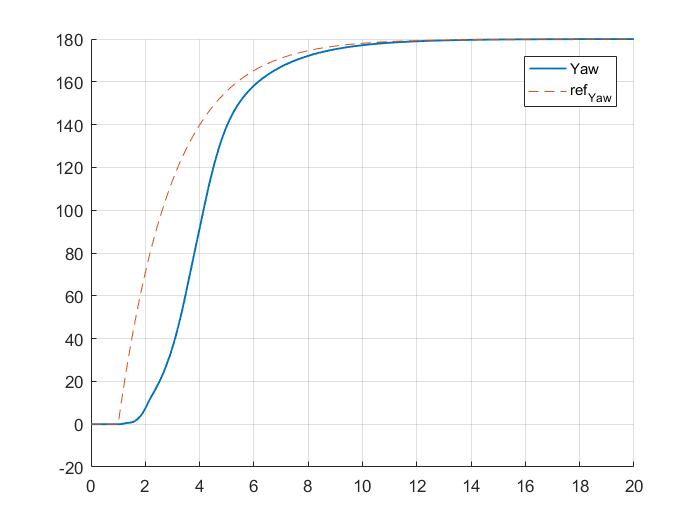
\includegraphics[width=\linewidth]{Plots_07_NonlinearModel_ReferenceTracking/05}
            \caption{Yaw}
        \end{subfigure}
        ~
        \begin{subfigure}[c]{0.3\linewidth}
            \centering
            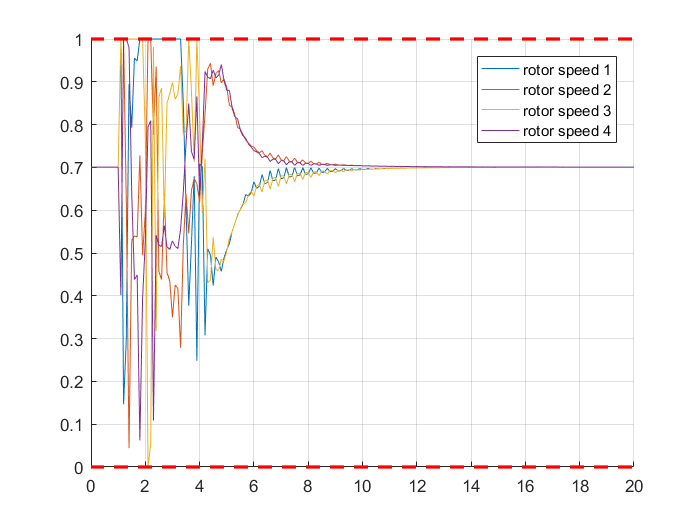
\includegraphics[width=\linewidth]{Plots_07_NonlinearModel_ReferenceTracking/06}
            \caption{Rotor Speeds}
        \end{subfigure}

        \begin{subfigure}[c]{0.3\linewidth}
            \centering
            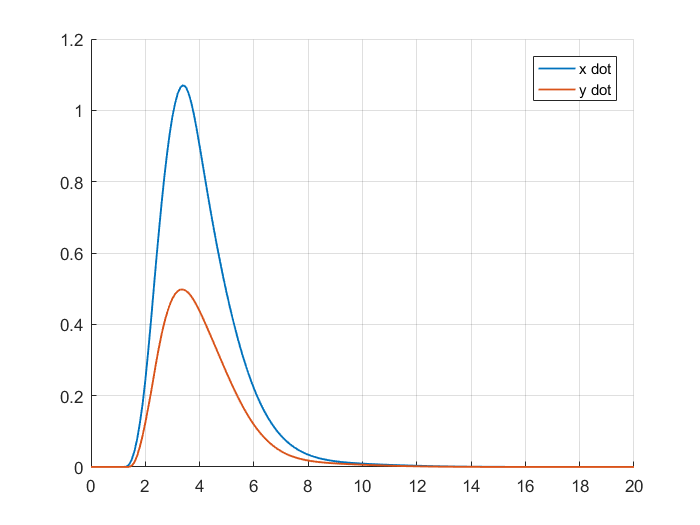
\includegraphics[width=\linewidth]{Plots_07_NonlinearModel_ReferenceTracking/07}
            \caption{xdot and ydot}
        \end{subfigure}
        ~
        \begin{subfigure}[c]{0.3\linewidth}
            \centering
            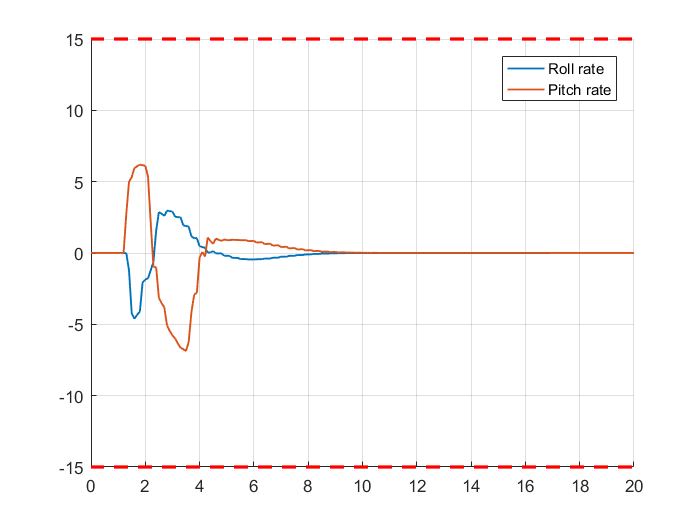
\includegraphics[width=\linewidth]{Plots_07_NonlinearModel_ReferenceTracking/08}
            \caption{Roll and Pitch rate}
        \end{subfigure}
        ~
        \begin{subfigure}[c]{0.3\linewidth}
            \centering
            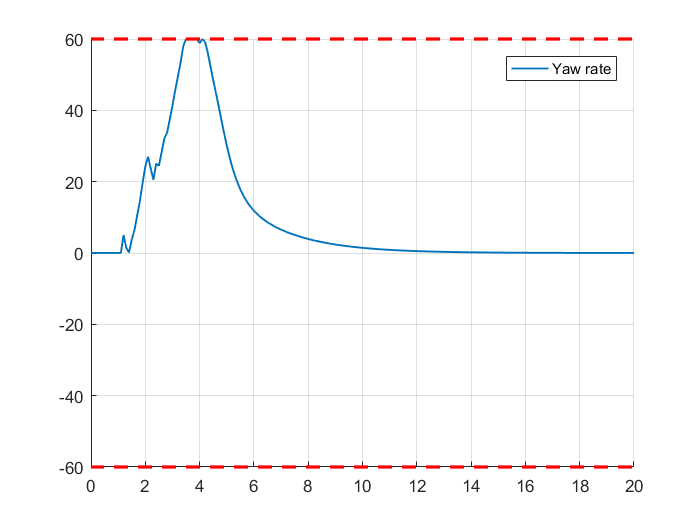
\includegraphics[width=\linewidth]{Plots_07_NonlinearModel_ReferenceTracking/09}
            \caption{Yaw rate}
        \end{subfigure}
        \caption{Reference tracking response of the nonlinear model.}
        \label{fig:nonlinear_reference_tracking_with_offset}
    \end{figure}
\end{enumerate}

% subsection first_simulation_of_the_nonlinear_model (end)


\subsection*{Offset free MPC} % (fold)
\label{sub:offset_free_mpc}

\begin{enumerate}
    \setcounter{enumi}{7}
    % 8.
    \item
	% 9.
	\item The response of the offset free tracking with a constant reference can be
    seen in Figure~\ref{fig:offset_free_tracking_with_constant}.
    \begin{figure}[ht]
        \centering
        \begin{subfigure}[c]{0.3\linewidth}
            \centering
            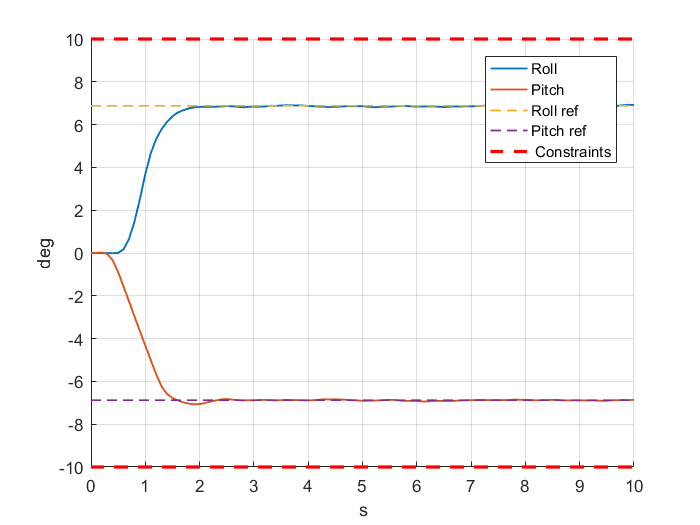
\includegraphics[width=\linewidth]{Plots_09_OffsetFreeTracking_Constant/01}
            \caption{Roll and Pitch}
        \end{subfigure}
        ~
        \begin{subfigure}[c]{0.3\linewidth}
            \centering
            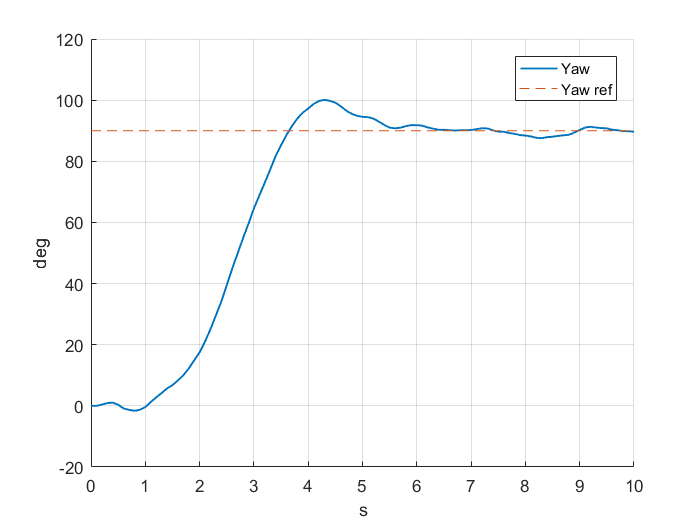
\includegraphics[width=\linewidth]{Plots_09_OffsetFreeTracking_Constant/02}
            \caption{Yaw}
        \end{subfigure}
        ~
        \begin{subfigure}[c]{0.3\linewidth}
            \centering
            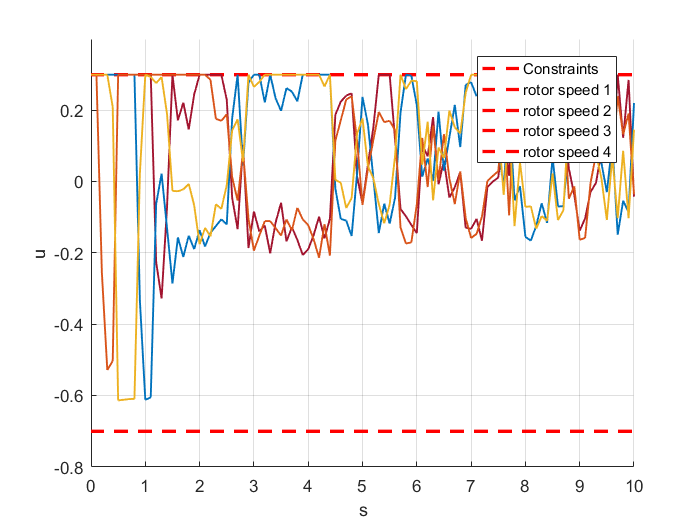
\includegraphics[width=\linewidth]{Plots_09_OffsetFreeTracking_Constant/03}
            \caption{Rotor Speeds}
        \end{subfigure}

        \begin{subfigure}[c]{0.3\linewidth}
            \centering
            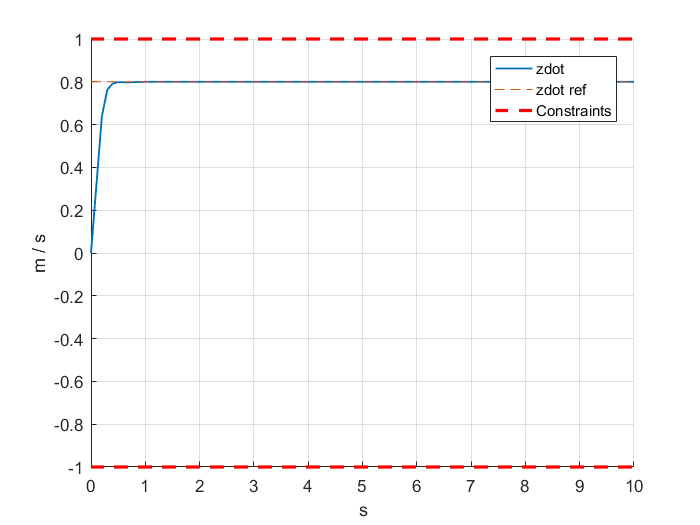
\includegraphics[width=\linewidth]{Plots_09_OffsetFreeTracking_Constant/04}
            \caption{zdot}
        \end{subfigure}
        ~
        \begin{subfigure}[c]{0.3\linewidth}
            \centering
            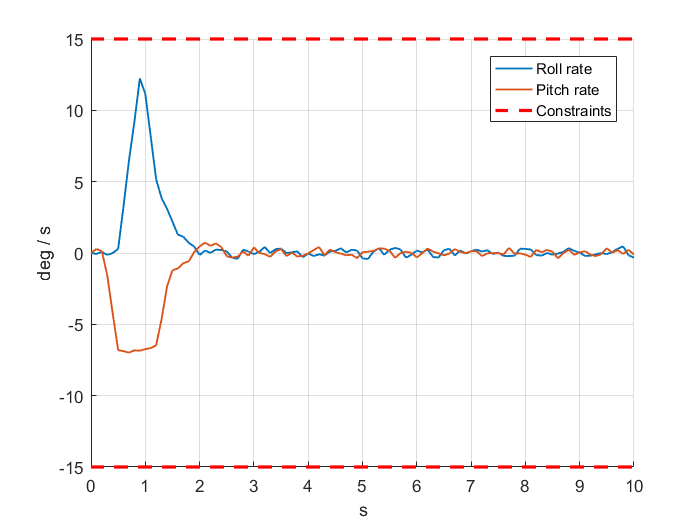
\includegraphics[width=\linewidth]{Plots_09_OffsetFreeTracking_Constant/05}
            \caption{Roll and Pitch rates}
        \end{subfigure}
        ~
        \begin{subfigure}[c]{0.3\linewidth}
            \centering
            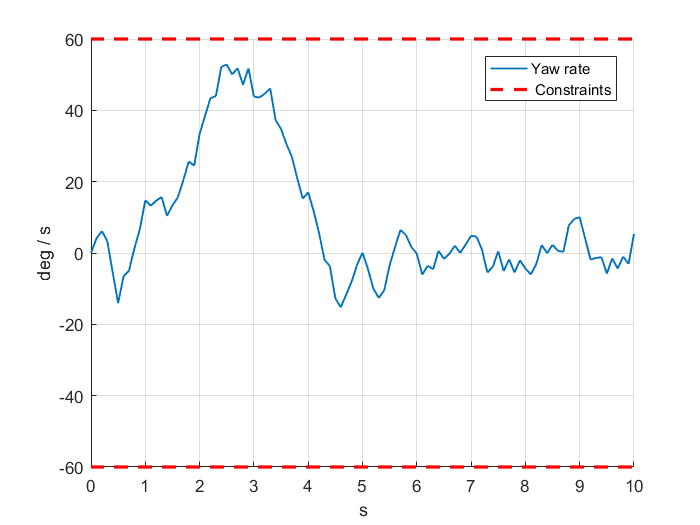
\includegraphics[width=\linewidth]{Plots_09_OffsetFreeTracking_Constant/06}
            \caption{Yaw rate}
        \end{subfigure}

        \begin{subfigure}[c]{0.3\linewidth}
            \centering
            \includegraphics[width=\linewidth]{Plots_09_OffsetFreeTracking_Constant/08}
            \caption{zdot disturbance}
        \end{subfigure}
        ~
        \begin{subfigure}[c]{0.3\linewidth}
            \centering
            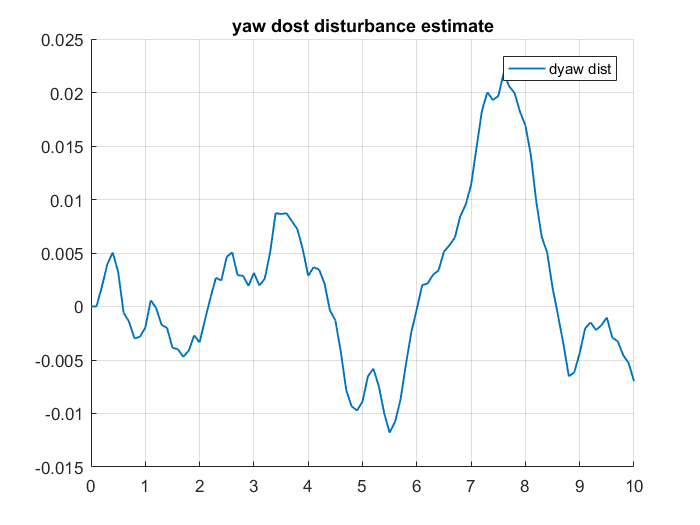
\includegraphics[width=\linewidth]{Plots_09_OffsetFreeTracking_Constant/09}
            \caption{Yawdot disturbance}
        \end{subfigure}
        ~
        \begin{subfigure}[c]{0.3\linewidth}
            \centering
            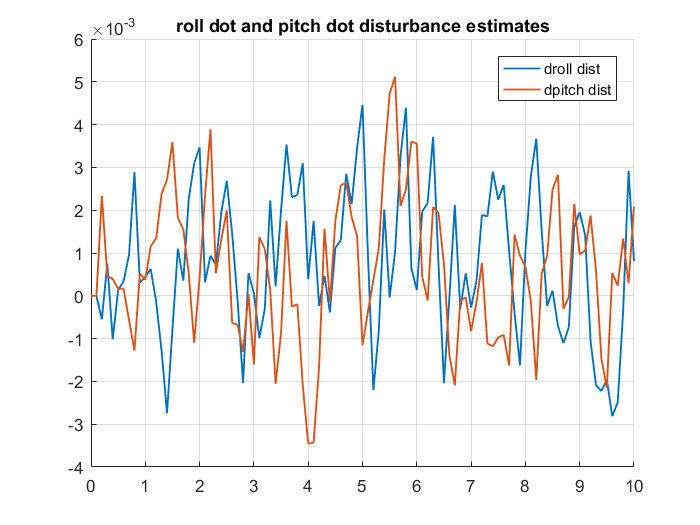
\includegraphics[width=\linewidth]{Plots_09_OffsetFreeTracking_Constant/10}
            \caption{Rolldot and Pitchdot disturbance}
        \end{subfigure}
        \caption{Offset-free tracking with a constant reference.}
        \label{fig:offset_free_tracking_with_constant}
    \end{figure}

    % 10.
    \item The response of the offset free tracking with a varying reference can be
    seen in Figure~\ref{fig:offset_free_tracking_with_varying}.
    \begin{figure}[ht]
        \centering
        \begin{subfigure}[c]{0.3\linewidth}
            \centering
            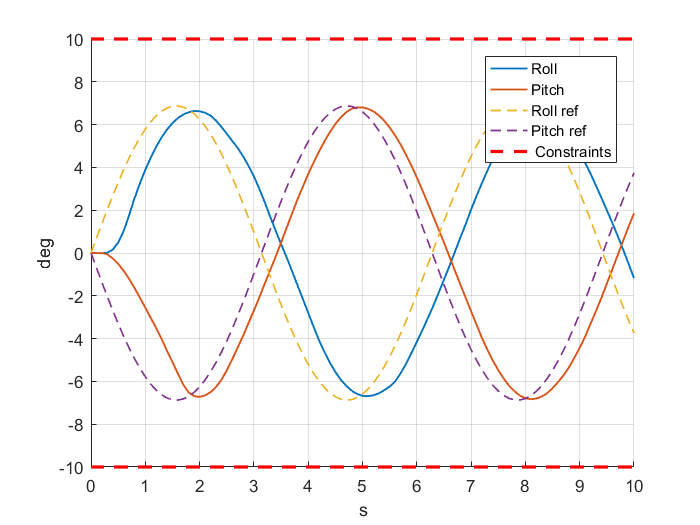
\includegraphics[width=\linewidth]{Plots_10_OffsetFreeTracking_Varying/01}
            \caption{Roll and Pitch}
        \end{subfigure}
        ~
        \begin{subfigure}[c]{0.3\linewidth}
            \centering
            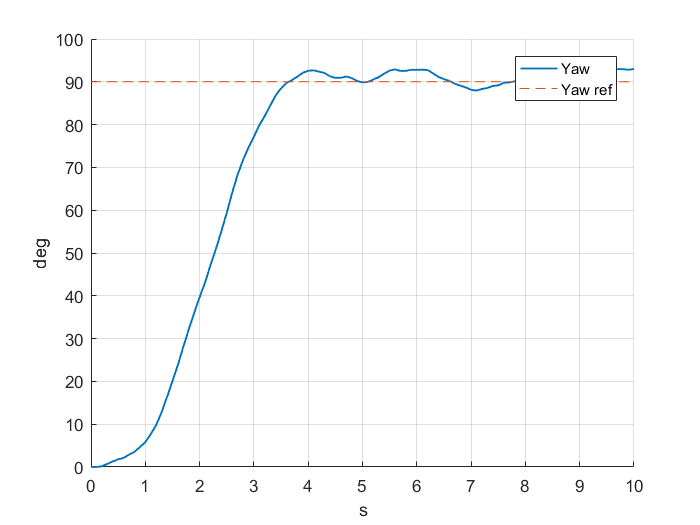
\includegraphics[width=\linewidth]{Plots_10_OffsetFreeTracking_Varying/02}
            \caption{Yaw}
        \end{subfigure}
        ~
        \begin{subfigure}[c]{0.3\linewidth}
            \centering
            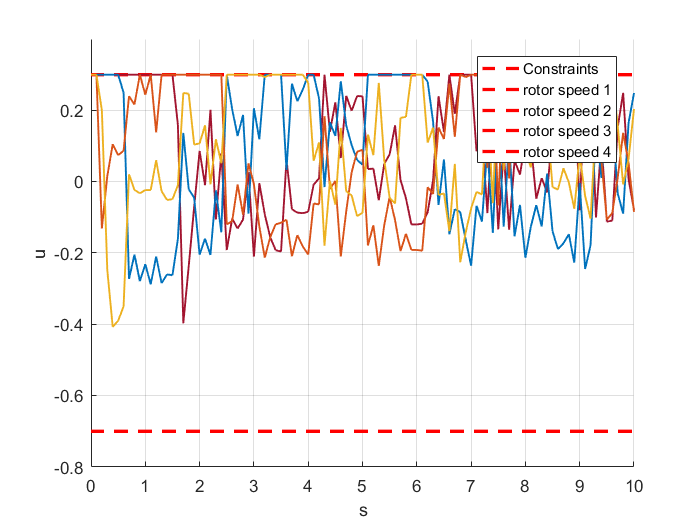
\includegraphics[width=\linewidth]{Plots_10_OffsetFreeTracking_Varying/03}
            \caption{Rotor Speeds}
        \end{subfigure}

        \begin{subfigure}[c]{0.3\linewidth}
            \centering
            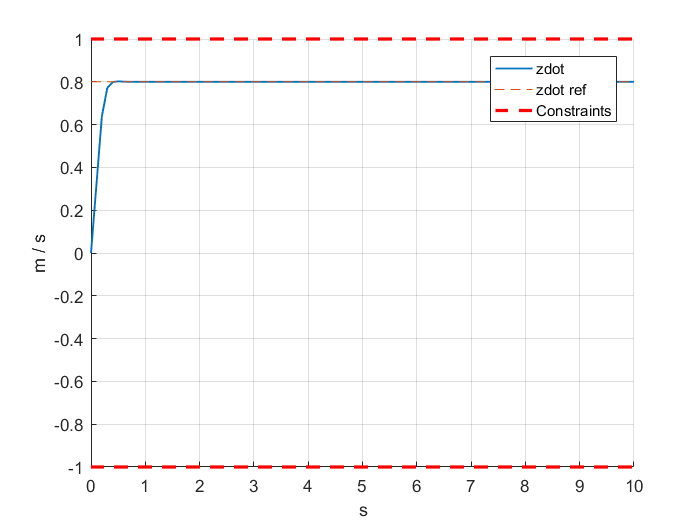
\includegraphics[width=\linewidth]{Plots_10_OffsetFreeTracking_Varying/04}
            \caption{zdot}
        \end{subfigure}
        ~
        \begin{subfigure}[c]{0.3\linewidth}
            \centering
            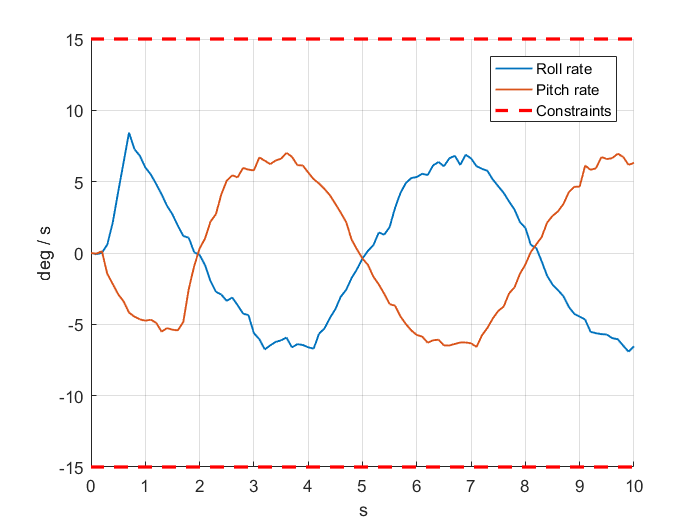
\includegraphics[width=\linewidth]{Plots_10_OffsetFreeTracking_Varying/05}
            \caption{Roll and Pitch rates}
        \end{subfigure}
        ~
        \begin{subfigure}[c]{0.3\linewidth}
            \centering
            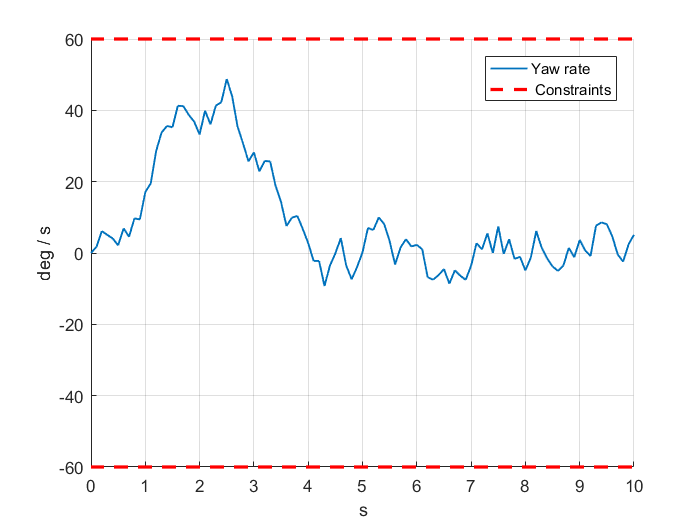
\includegraphics[width=\linewidth]{Plots_10_OffsetFreeTracking_Varying/06}
            \caption{Yaw rate}
        \end{subfigure}

        \begin{subfigure}[c]{0.3\linewidth}
            \centering
            \includegraphics[width=\linewidth]{Plots_10_OffsetFreeTracking_Varying/08}
            \caption{zdot disturbance}
        \end{subfigure}
        ~
        \begin{subfigure}[c]{0.3\linewidth}
            \centering
            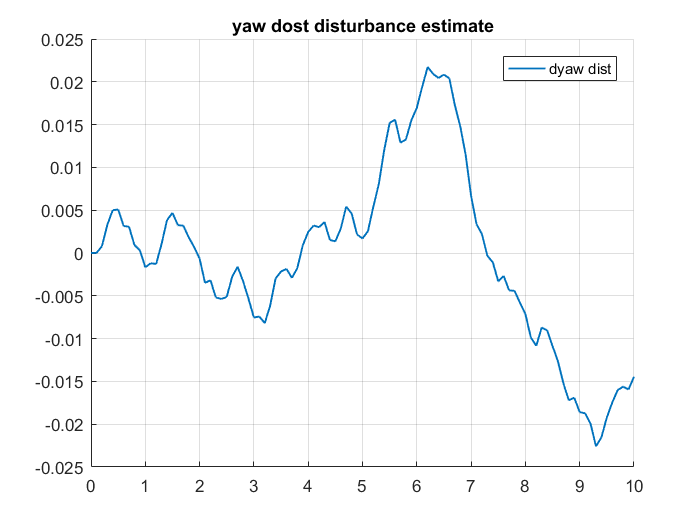
\includegraphics[width=\linewidth]{Plots_10_OffsetFreeTracking_Varying/09}
            \caption{Yawdot disturbance}
        \end{subfigure}
        ~
        \begin{subfigure}[c]{0.3\linewidth}
            \centering
            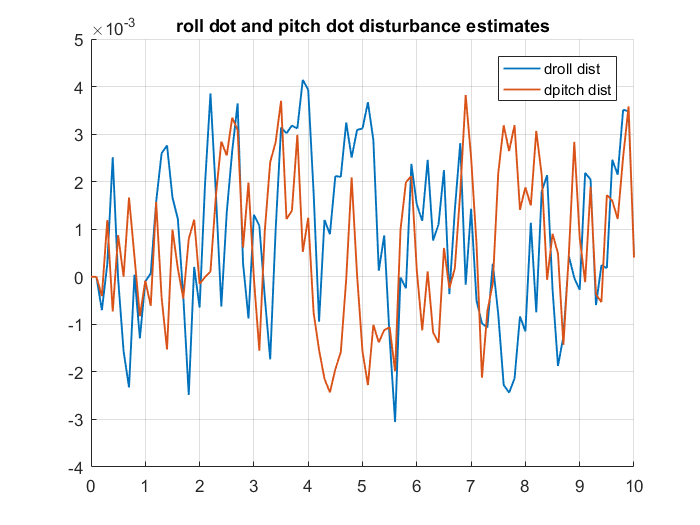
\includegraphics[width=\linewidth]{Plots_10_OffsetFreeTracking_Varying/10}
            \caption{Rolldot and Pitchdot disturbance}
        \end{subfigure}
        \caption{Offset-free tracking with a varying reference.}
        \label{fig:offset_free_tracking_with_varying}
    \end{figure}
    
\end{enumerate}

% subsection offset_free_mpc (end)


\subsection*{Simulation of the nonlinear model} % (fold)
\label{sub:simulation_of_the_nonlinear_model}

\begin{enumerate}
    \setcounter{enumi}{10}
    % 11.
    \item

    % 12.
    \item

    % 13.
    \item
\end{enumerate}

% subsection simulation_of_the_nonlinear_model (end)


\subsection*{Slew rate constraints} % (fold)
\label{sub:slew_rate_constraints}

\begin{enumerate}
    \setcounter{enumi}{13}
    % 14.
    \item
\end{enumerate}

% subsection slew_rate_constraints (end)


\subsection*{Soft Constraints} % (fold)
\label{sub:soft_constraints}

\begin{enumerate}
    \setcounter{enumi}{14}
    % 15.
    \item

    % 16.
    \item

\end{enumerate}

% subsection soft_constraints (end)


\subsection*{FORCES Pro} % (fold)
\label{sub:forces_pro}

\begin{enumerate}
    \setcounter{enumi}{16}
    % 17.
    \item
\end{enumerate}

% subsection forces_pro (end)

\end{document}
